این سامانه می‌تواند با استفاده از معماری چندلایه طراحی شود. این معماری قابلیت مقیاس‌پذیری و نگهداری مناسب را فراهم می‌کند. لایه‌های پیشنهادی به شرح زیر هستند:


	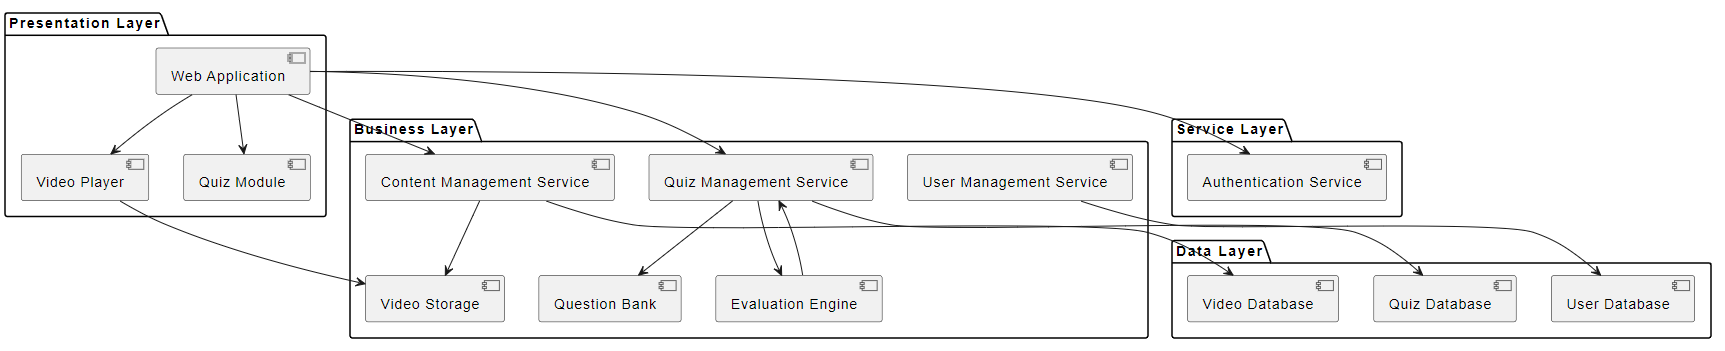
\includegraphics[width=1\linewidth]{screenshot001}


لایه Presentation مربوط به واسط کاربری است و تعامل کاربران با سیستم را مدیریت می‌کند.
 
لایه Business تمامی قوانین و منطق اصلی سیستم را اجرا می‌کند و به عنوان واسطه بین لایه نمایش و لایه سرویس عمل می‌کند.

لایه Service وظیفه ارائه API‌ ها و مدیریت ارتباط بین لایه کسب‌وکار و لایه داده را دارد. 

لایه Data وظیفه ذخیره و مدیریت داده‌ها را بر عهده دارد.



	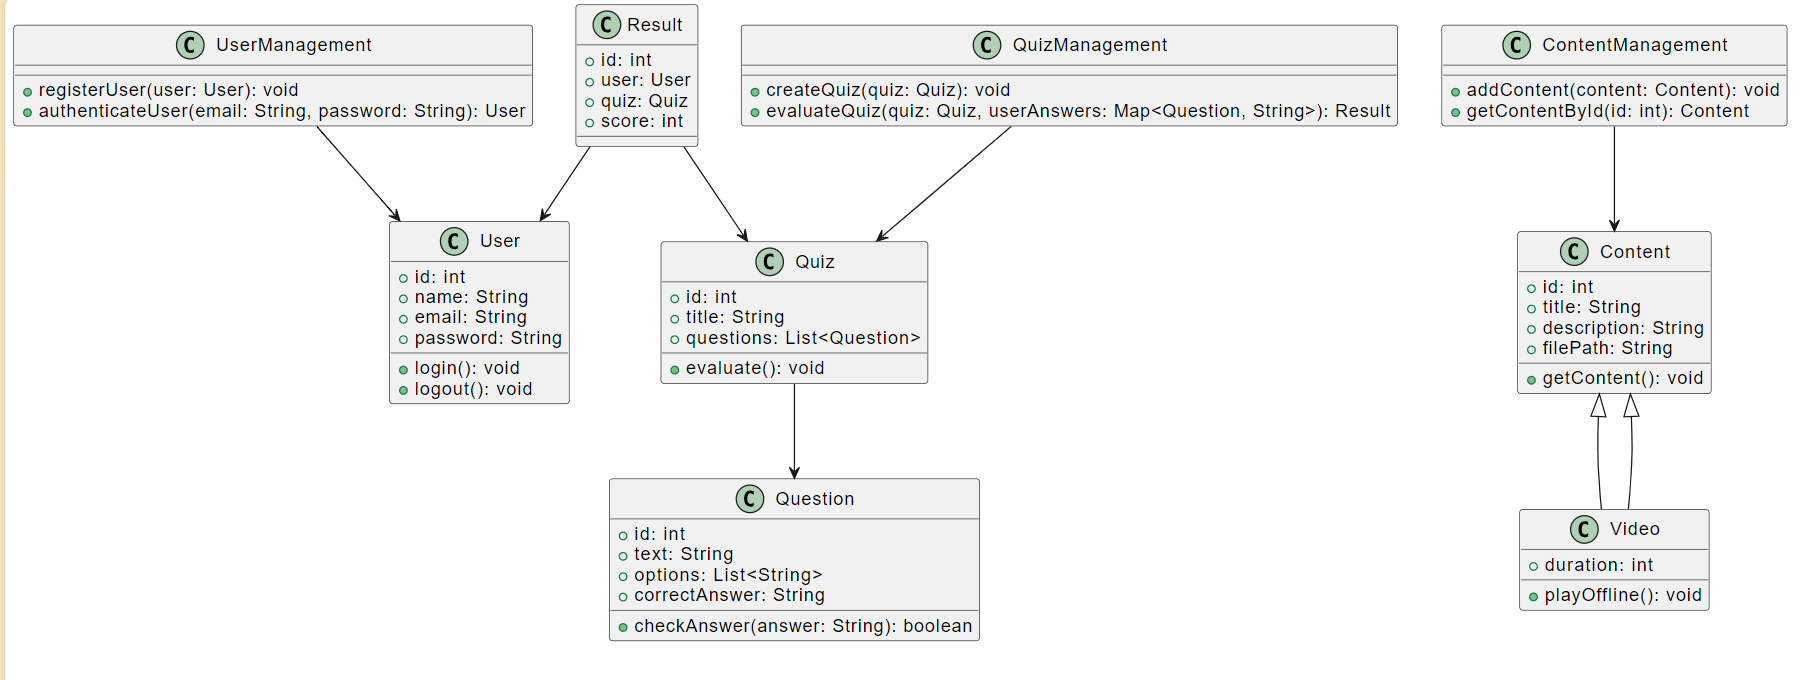
\includegraphics[width=1\linewidth]{screenshot002}



	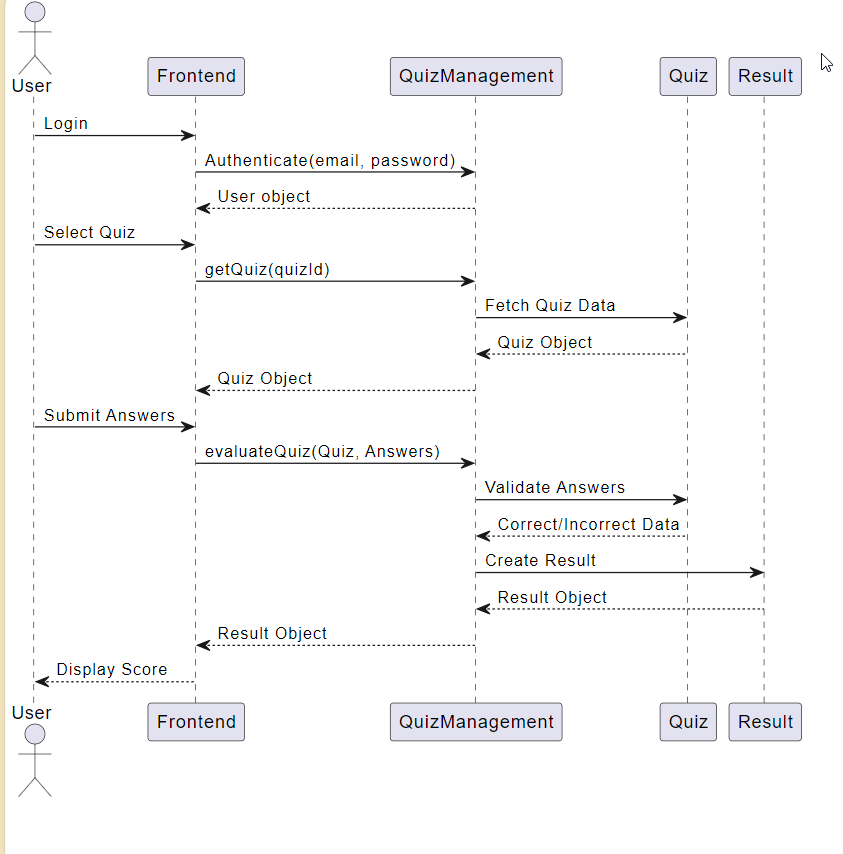
\includegraphics[width=0.5\linewidth]{screenshot003}
